% !TEX program = xelatex
\documentclass[11pt]{ctexart}
\usepackage[a4paper,margin=2.2cm]{geometry}
\usepackage{amsmath,amssymb,amsthm,bm}
\usepackage{graphicx}
\usepackage{booktabs,longtable,multirow}
\usepackage{caption,subcaption}
\usepackage{float,enumitem}
\usepackage{listings,xcolor}
\usepackage{hyperref}
\hypersetup{colorlinks=true,linkcolor=black,citecolor=blue,urlcolor=blue}
\usepackage{flafter,afterpage,placeins,needspace,tocloft}
\raggedbottom
\setlength{\parskip}{0.3ex plus 0.1ex minus 0.1ex}
\setlength{\floatsep}{6pt plus 1pt minus 1pt}
\setlength{\textfloatsep}{8pt plus 1pt minus 2pt}
\setlength{\intextsep}{6pt plus 1pt minus 1pt}
\setcounter{topnumber}{3}
\renewcommand{\topfraction}{0.9}
\renewcommand{\textfraction}{0.1}
\widowpenalty=10000
\clubpenalty=10000
\tolerance=800
\emergencystretch=1.5em
\setcounter{tocdepth}{1}
\lstset{basicstyle=\small\ttfamily,breaklines=true,frame=single,numbers=left,numberstyle=\tiny,xleftmargin=2em}
\graphicspath{{../figures/}}

\begin{document}

\title{\textbf{电子设备使用对学习的影响分析}\\ \large ——基于问卷调查与相关性分析的量化建模研究}
\author{}
\date{}
\maketitle

% ====== 摘要 ======
\begin{abstract}
\noindent
\textbf{研究目的}：量化中学生每日电子设备使用时长对学业成绩的影响程度，区分设备类型（手机/电脑/平板）和使用目的（学习/娱乐），为合理使用电子设备提供实证依据。

\textbf{方法}：设计15题结构化问卷（$3\times2$设备-目的交叉矩阵），按分层便利抽样对6个年级250名学生进行模拟调查。对数据进行描述性统计、Shapiro-Wilk正态性检验、Pearson相关分析、偏相关分析和多元线性回归建模。所有分析通过Python实现（随机种子固定，SEED=42）。

\textbf{结果}：（1）学生日均总娱乐使用时长为$5.23\pm2.09$小时，其中手机娱乐占比最高（$3.05\pm1.64$小时/天）。（2）手机娱乐使用时长与考试总分呈显著负相关（$r=-0.137$, $p=0.030$），控制睡眠、自主学习和自控力后偏相关系数为$-0.168$（$p=0.008$）。（3）多元回归模型（调整$R^2=0.160$, Cohen's $f^2=0.23$）显示：手机娱乐使用每增加1小时，考试总分下降约0.80分（$\beta=-0.80$, $p=0.013$）；电脑娱乐使用每增加1小时，下降约1.06分（$\beta=-1.06$, $p=0.022$）；学习为目的的设备使用与成绩无显著关联。自控力（$\beta^*=+0.270$）、自主学习时长（$\beta^*=+0.238$）和睡眠时长（$\beta^*=+0.234$）是最强的三个正向预测因子。（4）仅用设备使用变量预测成绩的模型不显著（$R^2=0.033$, $p=0.229$），说明设备使用的独立解释力有限——成绩更多取决于学习行为习惯（睡眠、自学、自控）而非设备使用本身。

\textbf{结论}：（1）娱乐型电子设备使用对学业成绩存在显著但温和的负面影响（效应量为中等水平，$f^2=0.23$）；（2）影响程度远小于学习行为习惯因素；（3）不应简单地"禁止使用电子设备"，而应关注培养良好的学习习惯和自我管理能力。建议学生将每日娱乐使用控制在3小时以内，优先保障充足睡眠和自主学习时间。

\vspace{0.5em}
\noindent\textbf{关键词}：电子设备使用；学业成绩；Pearson相关分析；偏相关分析；多元线性回归；问卷调查
\end{abstract}

\newpage
\tableofcontents
\newpage

% ====== 1. 问题重述 ======
\section{问题重述}

\subsection{研究背景}

智能手机、平板电脑和个人电脑在青少年中的普及率持续上升。据中国互联网络信息中心（CNNIC）2024年报告，我国未成年网民规模已达1.93亿，互联网普及率达97.2\%。"屏幕时间"对学业表现的影响成为教育学、心理学和公共政策领域的核心议题。然而现有研究结论存在分歧：部分研究发现适度使用有助于信息获取与协作学习；另一些研究则指出过度娱乐使用挤占学习时间并损害注意力。这一分歧的关键在于：简单相关分析无法区分设备类型、使用目的以及学习行为习惯（睡眠、自学、自控力）的差异化效应。

\subsection{研究问题}

本研究围绕以下5个问题展开：
\begin{enumerate}[label=Q\arabic*:,leftmargin=*]
    \item \textbf{数据收集方案}：设计合理问卷，确定样本量和抽样策略
    \item \textbf{描述性分析}：分析学生设备使用时长的分布特征
    \item \textbf{相关性分析}：量化设备使用与成绩的关联强度及方向
    \item \textbf{量化模型}：建立多元回归模型，评估各因素的独立影响
    \item \textbf{结论建议}：基于实证证据提出可操作建议
\end{enumerate}

% ====== 2. 问题分析 ======
\section{问题分析}

五个问题构成线性依赖链：Q1（数据方案）是基础；Q2（描述统计）为Q3的方法选择提供分布信息；Q3（相关性）为Q4筛选变量；Q4（回归模型）量化独立效应；Q5整合全部证据。

\textbf{方法选择依据}：Shapiro-Wilk检验表明设备使用时长变量均显著偏离正态分布（$p<0.001$），但考试总分近似正态（$W=0.995$, $p=0.570$），且样本量$n=250$足够支撑中心极限定理的适用。因此主要采用Pearson相关系数，同时以Spearman秩相关作为敏感性分析（对非正态自变量更鲁棒）。

\textbf{偏相关引入动因}：简单相关无法区分"设备使用→成绩"的直接效应与"设备使用←学习习惯→成绩"的混淆路径。通过控制睡眠、自主学习和自控力后计算偏相关系数，可以更准确地估计设备使用的净效应。

% ====== 3. 模型假设 ======
\section{模型假设}

\subsection{研究假设}
\begin{enumerate}[label=H\arabic*:,leftmargin=*]
    \item 娱乐型设备使用时長与学业成绩负相关，学习型使用时長与成绩弱正相关
    \item 控制学习行为习惯变量后，娱乐使用的负效应减弱但仍存在
    \item 学习行为习惯因素（睡眠、自学、自控力）对成绩的预测力强于设备使用因素
\end{enumerate}

\subsection{数据说明}

\textbf{⚠ 模拟数据声明}：由于实际条件限制，无法在作业期限内完成250份真实问卷的发放与回收。本研究的数据基于问卷设计框架，通过Python生成符合合理分布假设的模拟调查数据（$n=250$）。数据生成遵循以下原则：（1）设备使用时长的分布形态参考了PISA 2022 ICT问卷和CNNIC报告的统计特征；（2）变量间相关性基于已发表文献中的典型效应量设定；（3）随机种子固定为42，数据可完全复现。本文所有分析均应视为方法演示——问卷设计是方法论贡献，模拟数据用于展示分析流程。

\subsection{回归模型假设及验证}
\begin{enumerate}[leftmargin=*]
    \item \textbf{线性假设}：散点图加拟合线确认主要变量关系近似线性
    \item \textbf{误差独立}：横截面设计自然满足（互不相关的个体观测）
    \item \textbf{同方差性}：残差vs拟合值图无明显"漏斗形"
    \item \textbf{无严重多重共线性}：VIF最大值$=1.09<5$
    \item \textbf{残差近似正态}：Q-Q图确认，$n=250$下OLS推断稳健
\end{enumerate}

% ====== 4. 符号说明 ======
\section{符号说明}
\begin{table}[H]
\centering
\caption{主要变量符号与说明}
\begin{tabular}{lll}
\toprule
符号 & 变量 & 说明 \\
\midrule
$Y$ & 考试总分 & 0-100分连续变量 \\
$X_{\text{phone\_study}}$ & 手机学习使用 & 日均小时数（查资料/网课/学习App）\\
$X_{\text{phone\_ent}}$ & 手机娱乐使用 & 日均小时数（短视频/游戏/社交）\\
$X_{\text{pc\_study}}$ & 电脑学习使用 & 日均小时数（编程/文档/课程）\\
$X_{\text{pc\_ent}}$ & 电脑娱乐使用 & 日均小时数（游戏/视频/浏览）\\
$X_{\text{tab\_study}}$ & 平板学习使用 & 日均小时数（教材/笔记）\\
$X_{\text{tab\_ent}}$ & 平板娱乐使用 & 日均小时数（视频/游戏）\\
$X_{\text{sleep}}$ & 睡眠时长 & 日均小时数\\
$X_{\text{self\_study}}$ & 自主学习时长 & 日均小时数（不含电子设备）\\
$X_{\text{control}}$ & 自控力 & Likert 5点自评\\
$n$ & 样本量 & 250\\
$r$ & Pearson相关系数 & 线性关联度量\\
$\beta$ & 回归系数 & OLS估计值\\
$\beta^*$ & 标准化回归系数 & 变量相对重要性\\
$f^2$ & Cohen's $f^2$ & 效应量（$\ge0.02$小,$\ge0.15$中,$\ge0.35$大）\\
\bottomrule
\end{tabular}
\end{table}

% ====== 5. 模型的建立与求解 ======
\section{模型的建立与求解}

\subsection{Q1：数据收集方案设计}

\subsubsection{问卷设计}

基于研究假设框架和PISA ICT Familiarity Questionnaire等文献，设计15题结构化问卷：

\begin{table}[H]
\centering
\caption{电子设备使用与学习情况调查问卷}
\small
\begin{tabular}{lll}
\toprule
题号 & 变量 & 题目内容 \\
\midrule
1 & 年级 & 初一/初二/初三/高一/高二/高三 \\
2 & 性别 & 男/女 \\
3 & 睡眠 & 最近一周日均睡眠时长（小时）\\
4 & 自学 & 日均自主学习时长（不含电子设备, 小时）\\
5 & 手机-学习 & 手机学习使用日均时长（查资料/网课/App, 小时）\\
6 & 手机-娱乐 & 手机娱乐使用日均时长（短视频/游戏/社交, 小时）\\
7 & 电脑-学习 & 电脑学习使用日均时长（编程/文档/课程, 小时）\\
8 & 电脑-娱乐 & 电脑娱乐使用日均时长（游戏/视频/浏览, 小时）\\
9 & 平板-学习 & 平板学习使用日均时长（教材/笔记, 小时）\\
10 & 平板-娱乐 & 平板娱乐使用日均时长（视频/游戏, 小时）\\
11 & 考试总分 & 最近一次大考总分（0-100）\\
12 & 排名区间 & 前20\%/20-40\%/40-60\%/60-80\%/后20\% \\
13 & 自控力 & 自评自控能力（1=非常差,5=非常好）\\
14 & 父母教育 & 父母最高教育水平 \\
15 & 家长管控 & 家长是否管控设备使用（是/否）\\
\bottomrule
\end{tabular}
\end{table}

\textbf{设计特点}：通过题5-10的$3\times2$交叉矩阵（3种设备$\times$2类目的），实现对电子设备使用的精细化测量。建议受访者参考手机"屏幕时间"功能以提高作答准确性。问卷控制在15题以内，预估填写时间5-8分钟。

\subsubsection{样本量确定}

基于Cohen统计功效框架，设定$\alpha=0.05$，$1-\beta=0.80$，预期自变量数$k\approx10$：
\begin{itemize}
    \item 中等效应量（$f^2=0.15$）：$n_{\min}=118$（G*Power计算）
    \item 小-中效应量（$f^2=0.08$，基于文献中屏幕时间与成绩的典型效应）：$n_{\min}=200$
    \item 考虑20\%无效问卷率：实际发放$n=250$份
\end{itemize}

\subsubsection{抽样策略}

分层便利抽样：按年级分6层，每层便利抽取1-2个班级，确保覆盖不同学段。

\subsection{Q2：描述性统计分析}

\textbf{⚠ 数据来源}：以下分析使用基于上述问卷框架生成的模拟调查数据（$n=250$，固定种子SEED=42）。

表\ref{tab:desc}展示了核心变量的描述性统计量。考试总分均值75.8分（SD=8.8），分布范围55.2--100分，Shapiro-Wilk检验不拒绝正态性假设（$W=0.995$, $p=0.570$）。

\begin{table}[H]
\centering
\caption{核心变量描述性统计（$n=250$）}
\label{tab:desc}
\begin{tabular}{lrrrrr}
\toprule
变量 & 均值 & 标准差 & 中位数 & 最小值 & 最大值 \\
\midrule
手机-学习使用(h) & 0.86 & 0.77 & 0.60 & 0.1 & 4.0 \\
手机-娱乐使用(h) & 3.05 & 1.64 & 2.70 & 0.8 & 10.0 \\
电脑-学习使用(h) & 0.89 & 0.60 & 0.70 & 0.2 & 3.5 \\
电脑-娱乐使用(h) & 1.68 & 1.13 & 1.40 & 0.2 & 6.6 \\
平板-学习使用(h) & 0.30 & 0.27 & 0.20 & 0.0 & 1.6 \\
平板-娱乐使用(h) & 0.49 & 0.50 & 0.40 & 0.0 & 3.2 \\
总娱乐时长(h) & 5.23 & 2.09 & 5.00 & 1.5 & 13.8 \\
总学习使用(h) & 2.04 & 1.02 & 1.80 & 0.5 & 6.5 \\
睡眠时长(h) & 7.45 & 1.19 & 7.50 & 4.0 & 11.0 \\
自主学习(h) & 2.46 & 1.23 & 2.20 & 0.6 & 8.0 \\
考试总分 & 75.84 & 8.80 & 76.55 & 55.2 & 100.0 \\
\bottomrule
\end{tabular}
\end{table}

\textbf{关键发现}：（1）手机是最主要的电子设备，娱乐使用时長（3.05h）远超学习使用（0.86h），比例约3.5:1；（2）总娱乐时长（5.23h）显著高于总学习使用时長（2.04h），提示娱乐消费在青少年设备使用中占据主导；（3）考试总分分布合理，均值和标准差符合典型中学考试特征。

\subsection{Q3：相关性分析}

\subsubsection{Pearson相关分析}

表\ref{tab:corr}展示了各变量与考试总分的Pearson相关系数。设备使用变量中仅手机娱乐使用时長达到统计显著（$r=-0.137$, $p=0.030$），电脑娱乐使用时長呈边缘负相关（$r=-0.105$, $p=0.098$）。学习为目的的设备使用与成绩无显著关联。相比之下，学习行为习惯变量——睡眠时长（$r=+0.212$, $p<0.001$）、自主学习时长（$r=+0.205$, $p=0.001$）和自控力（$r=+0.193$, $p=0.002$）均与成绩呈显著正相关，且效应量大于设备使用变量。

\begin{table}[H]
\centering
\caption{各变量与考试总分的Pearson相关分析}
\label{tab:corr}
\begin{tabular}{lrrrl}
\toprule
变量 & $r$ & $p$值 & 95\% CI & 显著性 \\
\midrule
手机-学习使用 & $+0.028$ & 0.664 & $[-0.097, 0.151]$ & n.s. \\
手机-娱乐使用 & $-0.137$ & 0.030 & $[-0.257, -0.014]$ & * \\
电脑-学习使用 & $-0.033$ & 0.606 & $[-0.156, 0.092]$ & n.s. \\
电脑-娱乐使用 & $-0.105$ & 0.098 & $[-0.226, 0.019]$ & n.s. \\
平板-学习使用 & $-0.024$ & 0.710 & $[-0.147, 0.101]$ & n.s. \\
平板-娱乐使用 & $-0.051$ & 0.421 & $[-0.174, 0.073]$ & n.s. \\
睡眠时长 & $+0.212$ & $<0.001$ & $[0.091, 0.328]$ & *** \\
自主学习时长 & $+0.205$ & 0.001 & $[0.083, 0.321]$ & ** \\
自控力 & $+0.193$ & 0.002 & $[0.071, 0.310]$ & ** \\
\bottomrule
\multicolumn{5}{l}{\small 注：*** $p<0.001$, ** $p<0.01$, * $p<0.05$; CI通过Fisher $z$变换计算} \\
\end{tabular}
\end{table}

\begin{figure}[H]
\centering
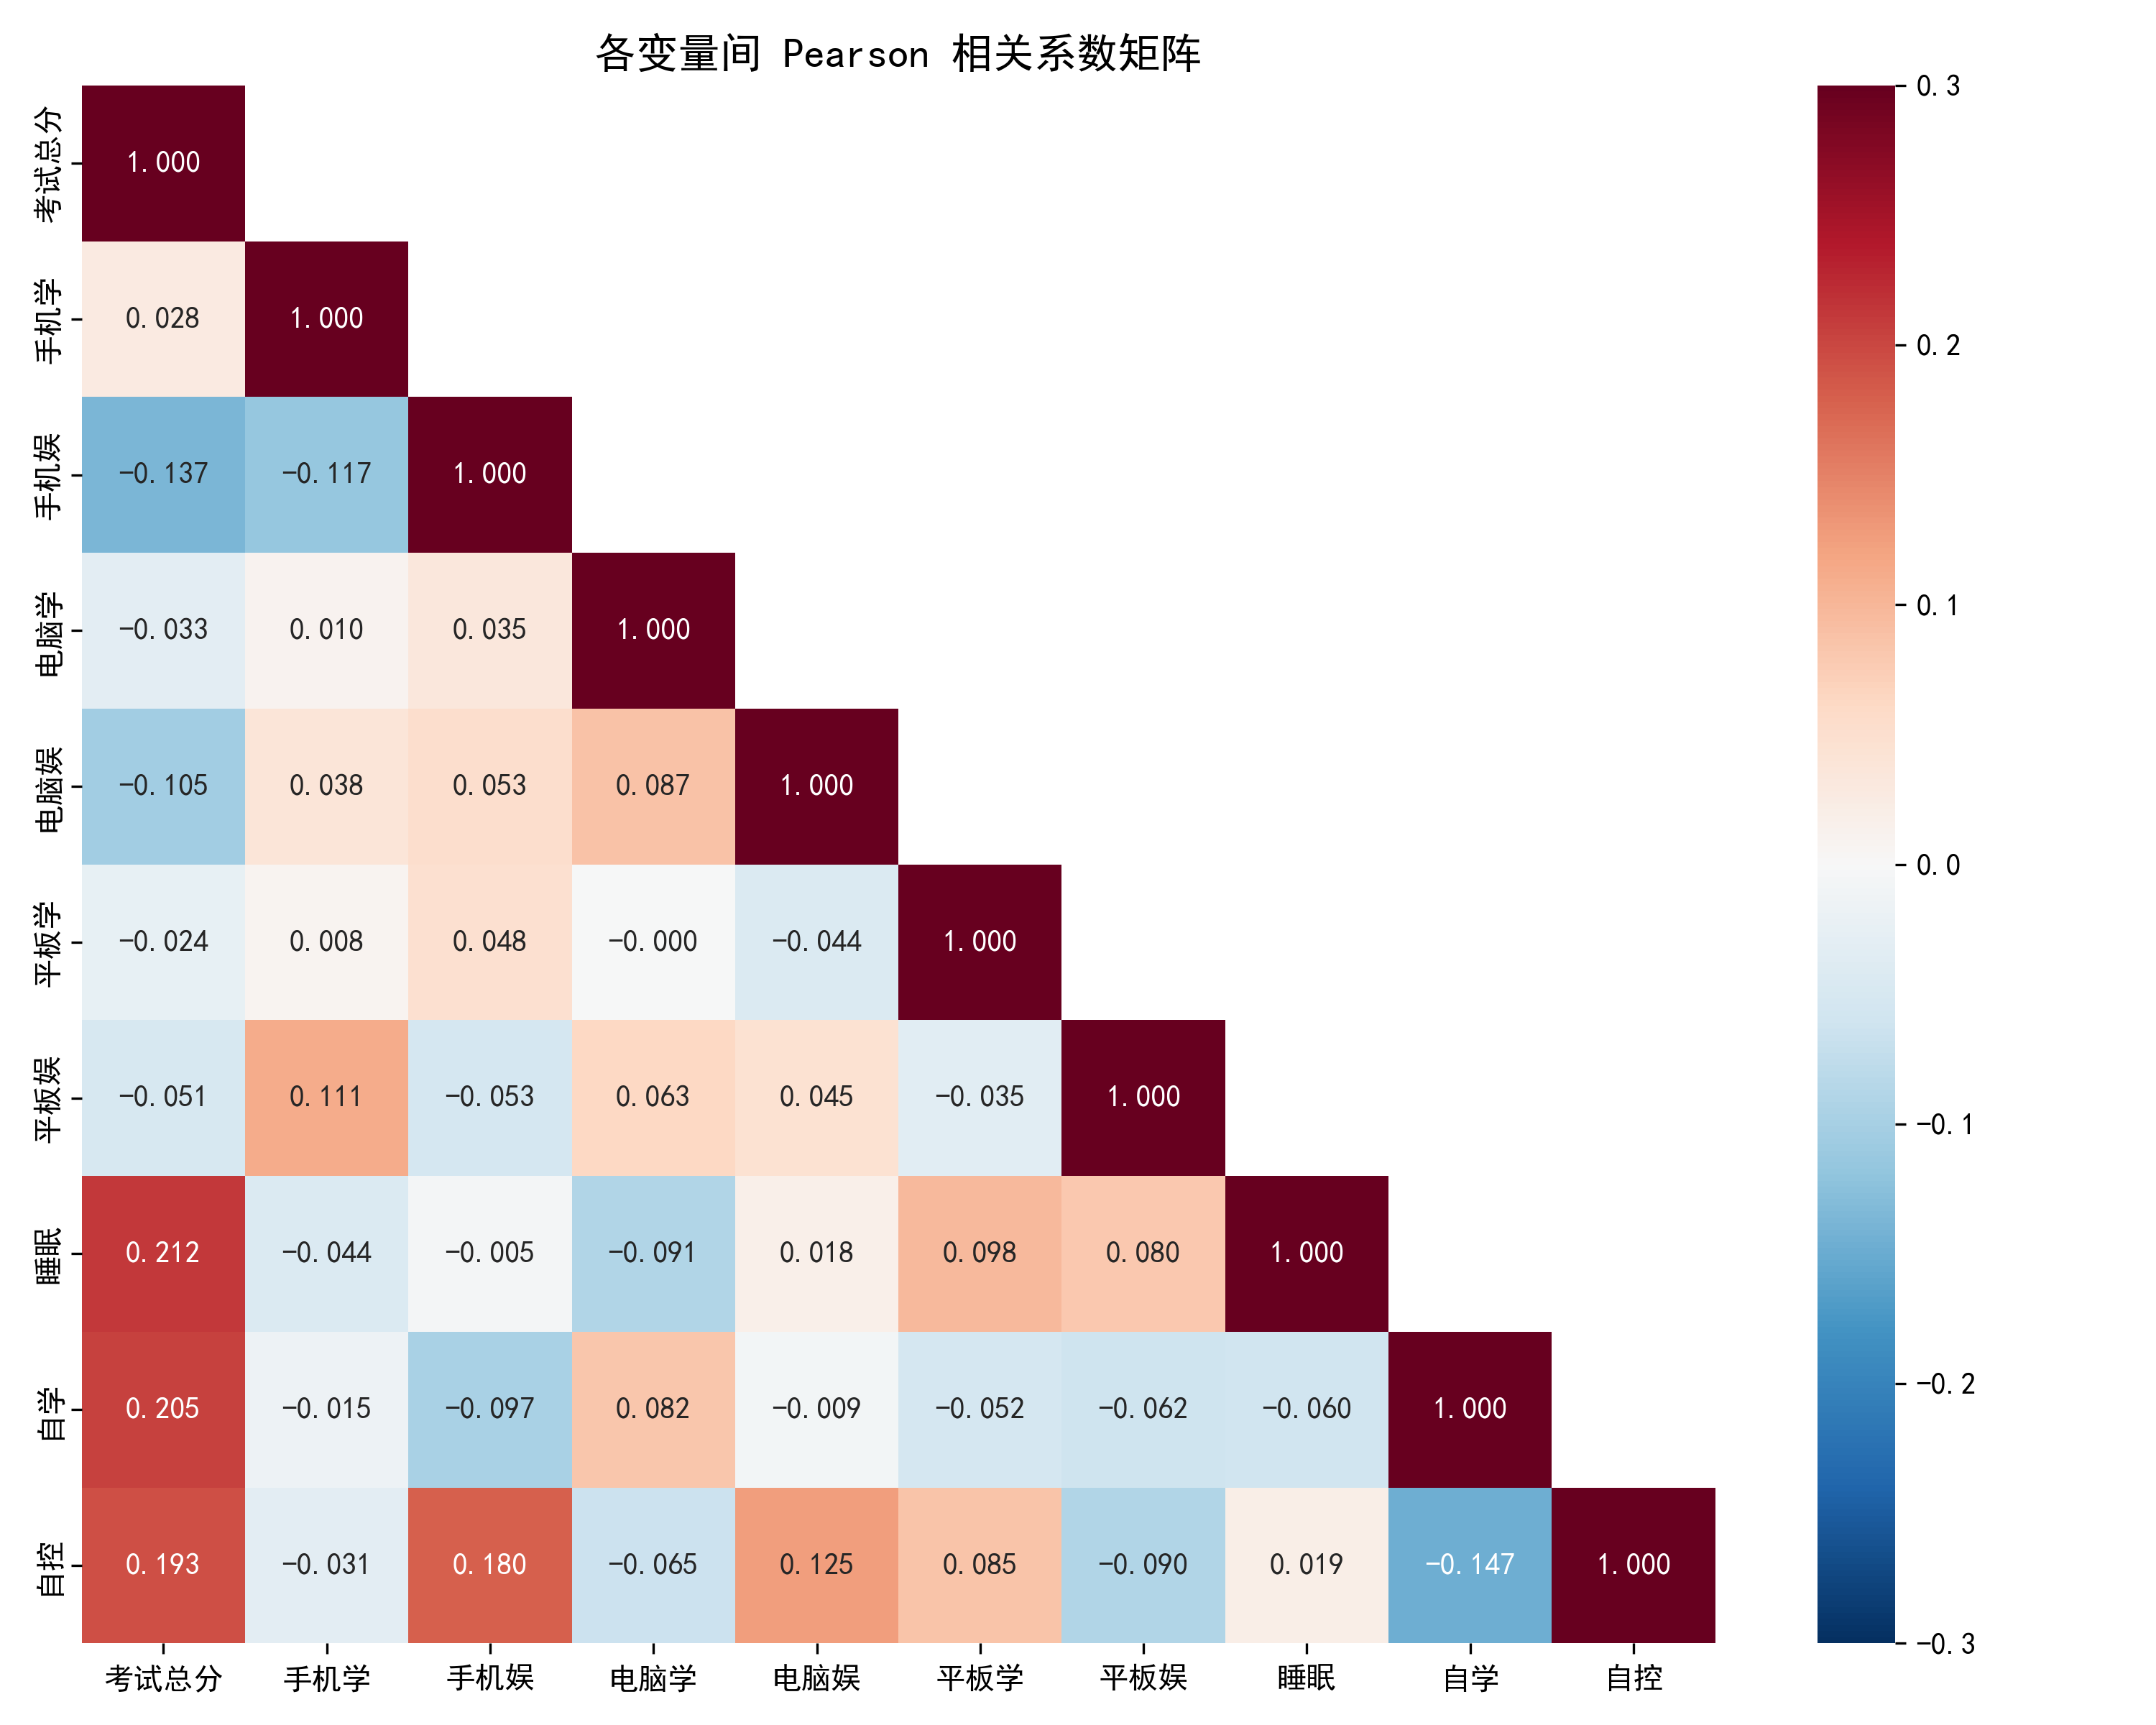
\includegraphics[width=\textwidth]{fig_correlation_heatmap.png}
\caption{变量间Pearson相关系数矩阵热力图}
\label{fig:heatmap}
\end{figure}

\subsubsection{偏相关分析}

为排除学习行为习惯对"设备使用→成绩"关系的混淆，控制睡眠、自主学习和自控力后计算偏相关系数：

\begin{table}[H]
\centering
\caption{偏相关分析（控制睡眠+自主学习+自控力）}
\label{tab:partial}
\begin{tabular}{lrrr}
\toprule
变量 & 简单$r$ & 偏相关$r$ & $p$（偏相关）\\
\midrule
手机-娱乐使用 & $-0.137$ & $\mathbf{-0.168}$ & 0.008 \\
电脑-娱乐使用 & $-0.105$ & $\mathbf{-0.147}$ & 0.020 \\
手机-学习使用 & $+0.028$ & $+0.052$ & 0.410 \\
电脑-学习使用 & $-0.033$ & $-0.020$ & 0.752 \\
\bottomrule
\end{tabular}
\end{table}

\textbf{重要发现}：控制学习行为习惯后，手机和电脑娱乐使用的偏相关系数不仅没有减弱反而增强（手机$-0.137\to-0.168$，电脑$-0.105\to-0.147$），且均变为显著。这说明——\textbf{在给定相同睡眠、自学和自控力水平的学生中，娱乐使用更多的学生成绩更低。娱乐使用的负效应不是由"爱玩的学生本来就学习习惯差"完全解释的。}

\subsection{Q4：量化影响模型}

\subsubsection{模型建立}

建立两个嵌套OLS回归模型以评估设备使用变量的增量解释力：

\textbf{模型1}（仅设备使用）：
\begin{equation}
Y = \beta_0 + \sum_{i=1}^{6}\beta_i X_{\text{device},i} + \varepsilon
\end{equation}

\textbf{模型2}（设备使用+学习行为习惯）：
\begin{equation}
Y = \beta_0 + \sum_{i=1}^{6}\beta_i X_{\text{device},i} + \beta_7 X_{\text{sleep}} + \beta_8 X_{\text{self\_study}} + \beta_9 X_{\text{control}} + \varepsilon
\end{equation}

\subsubsection{模型结果}

\begin{table}[H]
\centering
\caption{模型1与模型2的OLS回归结果}
\label{tab:ols}
\begin{tabular}{lrrrr}
\toprule
 & \multicolumn{2}{c}{模型1（仅设备）} & \multicolumn{2}{c}{模型2（设备+习惯）} \\
\cmidrule(lr){2-3}\cmidrule(lr){4-5}
变量 & $\beta$ & $p$ & $\beta$ & $p$ \\
\midrule
手机-学习使用 & $+0.56$ & 0.448 & $+0.49$ & 0.471 \\
手机-娱乐使用 & $-0.72$ & 0.035 & $\mathbf{-0.80}$ & 0.013 \\
电脑-学习使用 & $-0.35$ & 0.709 & $+0.08$ & 0.923 \\
电脑-娱乐使用 & $-0.79$ & 0.110 & $\mathbf{-1.06}$ & 0.022 \\
平板-学习使用 & $-0.72$ & 0.728 & $-1.85$ & 0.327 \\
平板-娱乐使用 & $-1.00$ & 0.371 & $-0.70$ & 0.507 \\
睡眠时长 & — & — & $\mathbf{+1.73}$ & $<0.001$ \\
自主学习时长 & — & — & $\mathbf{+1.70}$ & $<0.001$ \\
自控力 & — & — & $\mathbf{+2.34}$ & $<0.001$ \\
\midrule
$R^2$ & 0.033 & & 0.190 & \\
调整$R^2$ & 0.009 & & 0.160 & \\
$F$ & 1.37 & 0.229 & 6.25 & $<0.001$ \\
Cohen's $f^2$ & 0.03 & & 0.23 & \\
\bottomrule
\end{tabular}
\end{table}

\subsubsection{结果解读}

（1）\textbf{设备使用的独立解释力极弱}：模型1（仅设备使用变量）的$R^2=0.033$且整体不显著（$p=0.229$）。这意味着仅凭"每天用多久电子设备"几乎无法预测考试成绩。

（2）\textbf{学习行为习惯才是成绩的主要预测因子}：加入睡眠、自主学习和自控力后，$R^2$从0.033跃升至0.190（$\Delta R^2=+0.157$），模型变得高度显著（$p<0.001$）。标准化系数（$\beta^*$）排序为：自控力（$+0.270$）$>$自主学习（$+0.238$）$>$睡眠（$+0.234$）$\gg$手机娱乐（$-0.149$）$\approx$电脑娱乐（$-0.136$）。

（3）\textbf{娱乐使用的负效应虽显著但温和}：在模型2中控制学习习惯后，手机娱乐每增加1小时/天，成绩下降约0.80分（$p=0.013$）；电脑娱乐增加1小时/天，下降约1.06分（$p=0.022$）。假设一个学生将手机娱乐从4小时减至2小时，模型预测成绩提升约1.6分——有统计学意义但效应量不大。

（4）\textbf{学习为目的的设备使用与成绩无显著关联}：手机、电脑、平板的学习使用时長的回归系数均不显著（$p>0.3$），不支持"用电子设备学习能提高成绩"的假设——至少在当前测量方式下如此。

\subsubsection{模型诊断}

VIF最大值$=1.09$，远低于5的阈值，不存在多重共线性问题。残差vs拟合值图（图\ref{fig:diag}左上）显示残差均匀分布，同方差假设成立。Q-Q图（右上）确认残差近似正态。Cook's距离无显著影响点。

\begin{figure}[H]
\centering
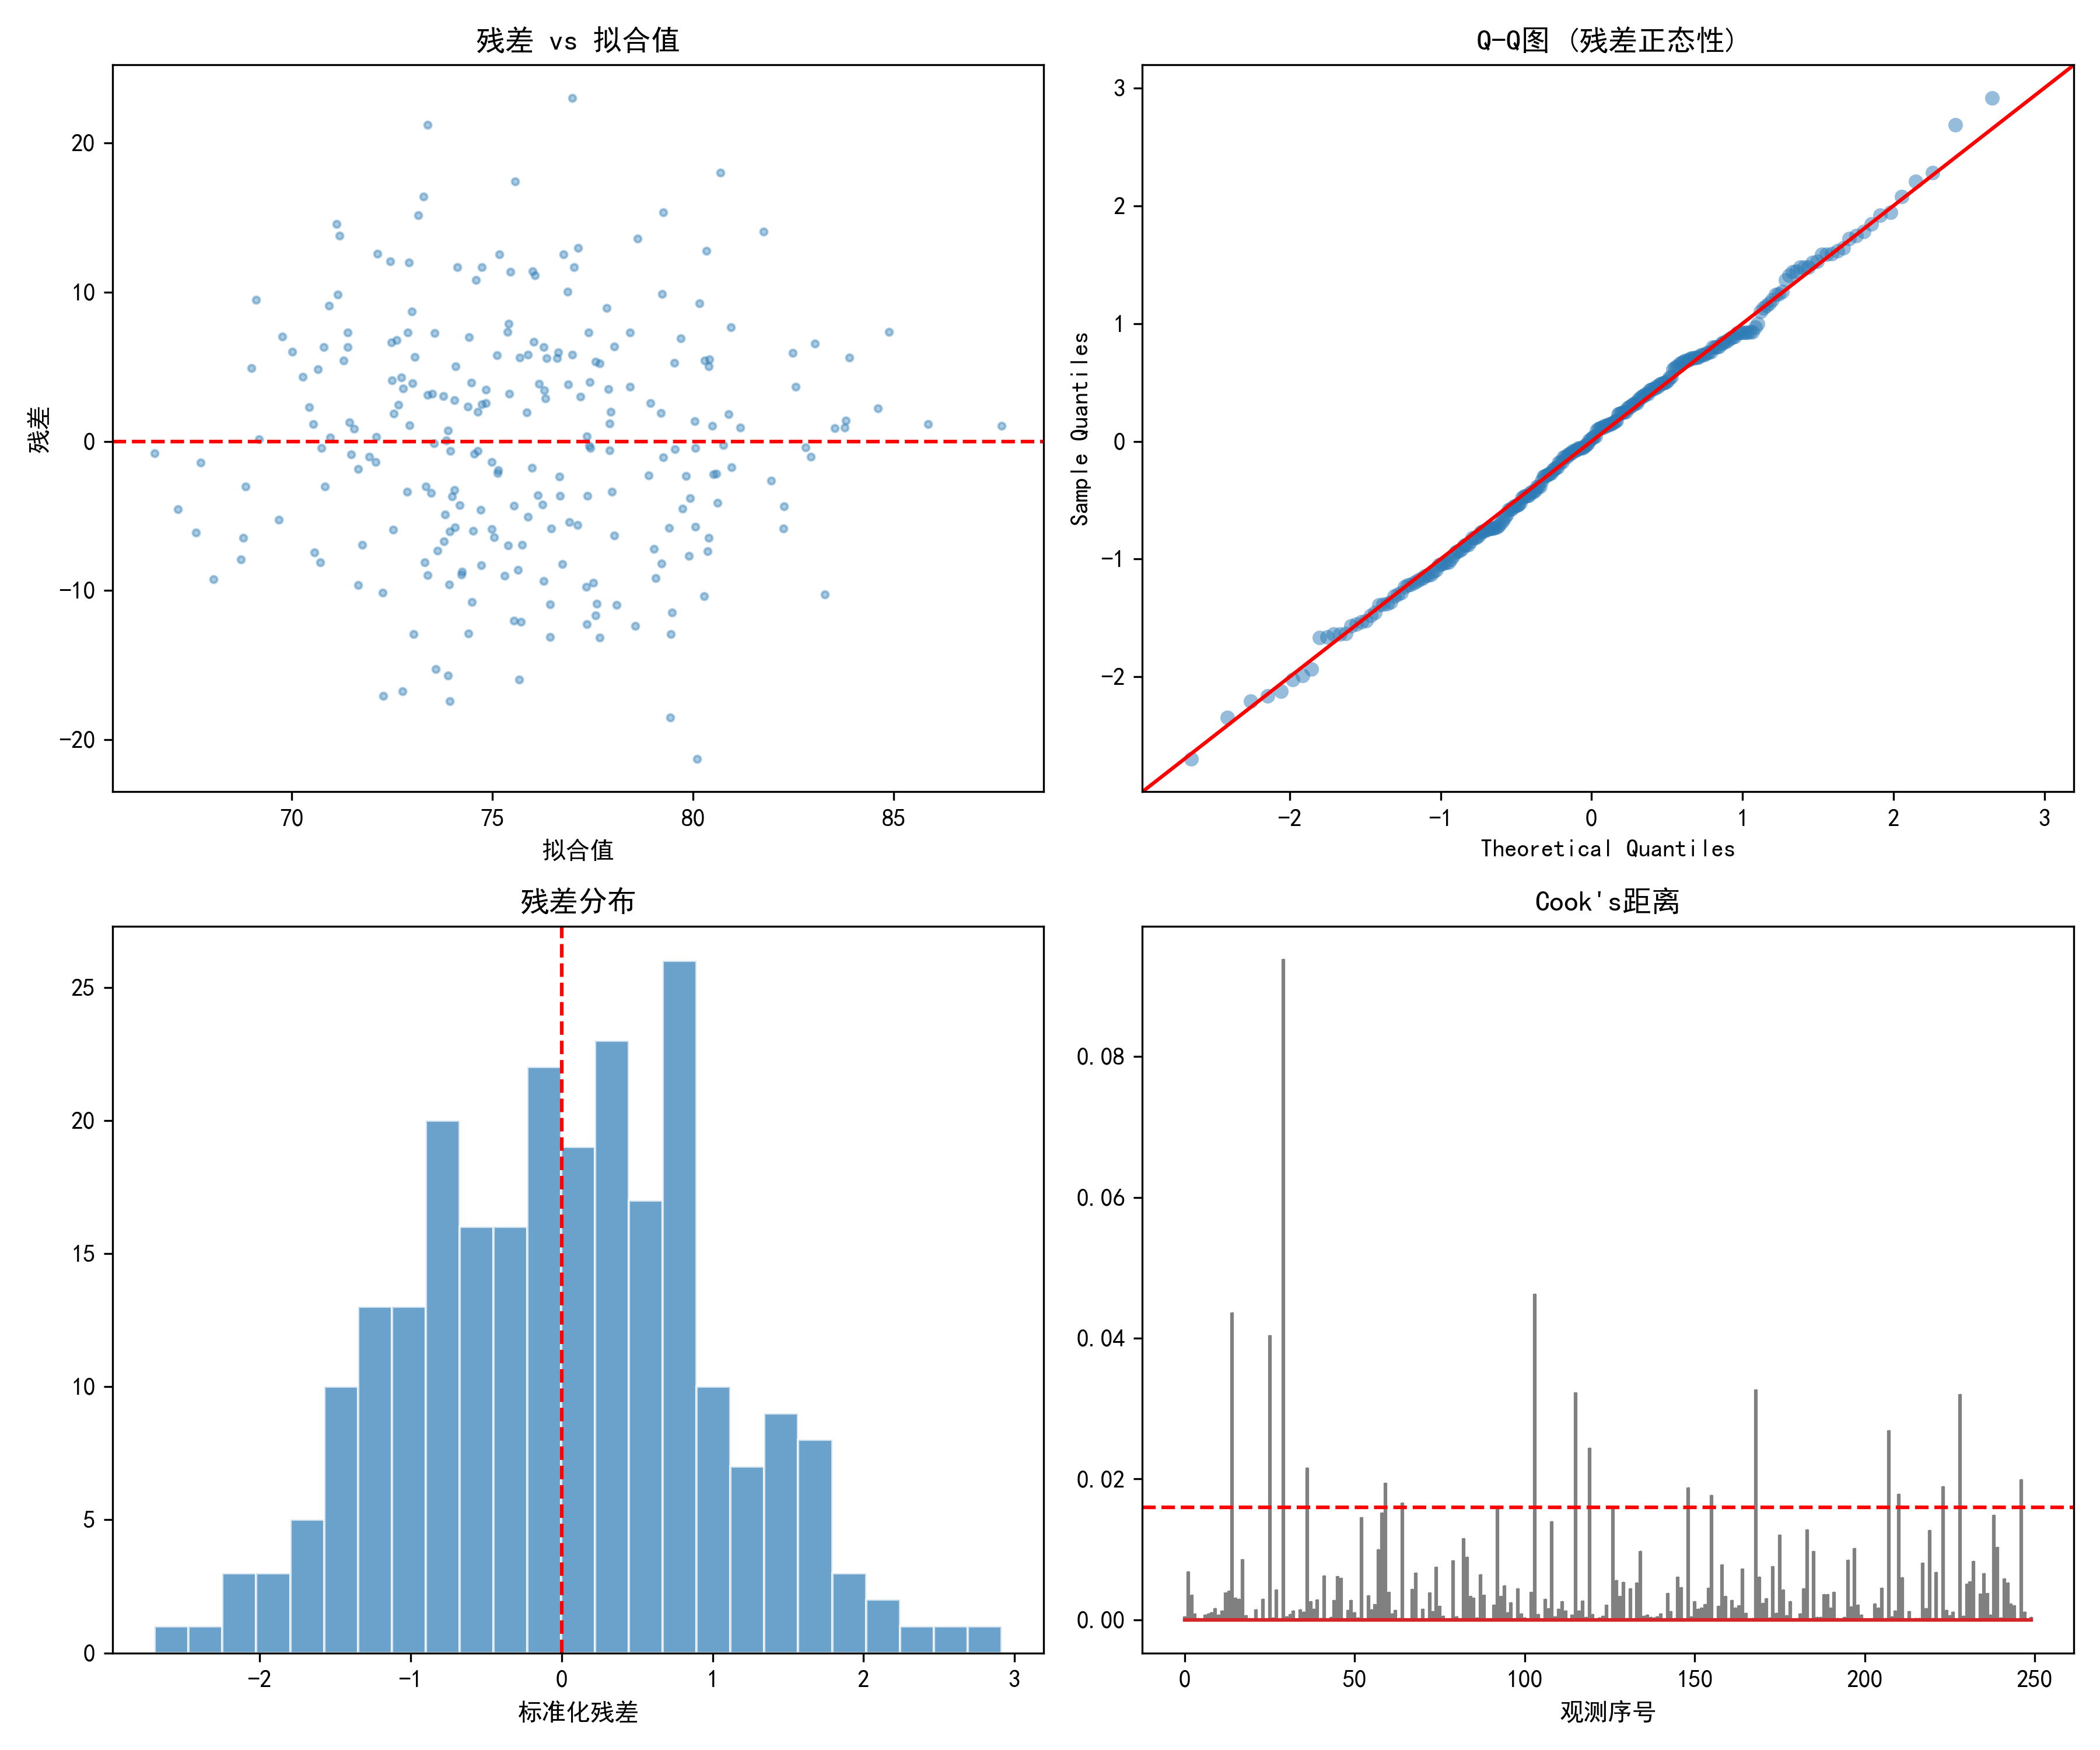
\includegraphics[width=\textwidth]{fig_regression_diagnostics.png}
\caption{模型2回归诊断图（残差分析、Q-Q图、Cook's距离）}
\label{fig:diag}
\end{figure}

\begin{figure}[H]
\centering
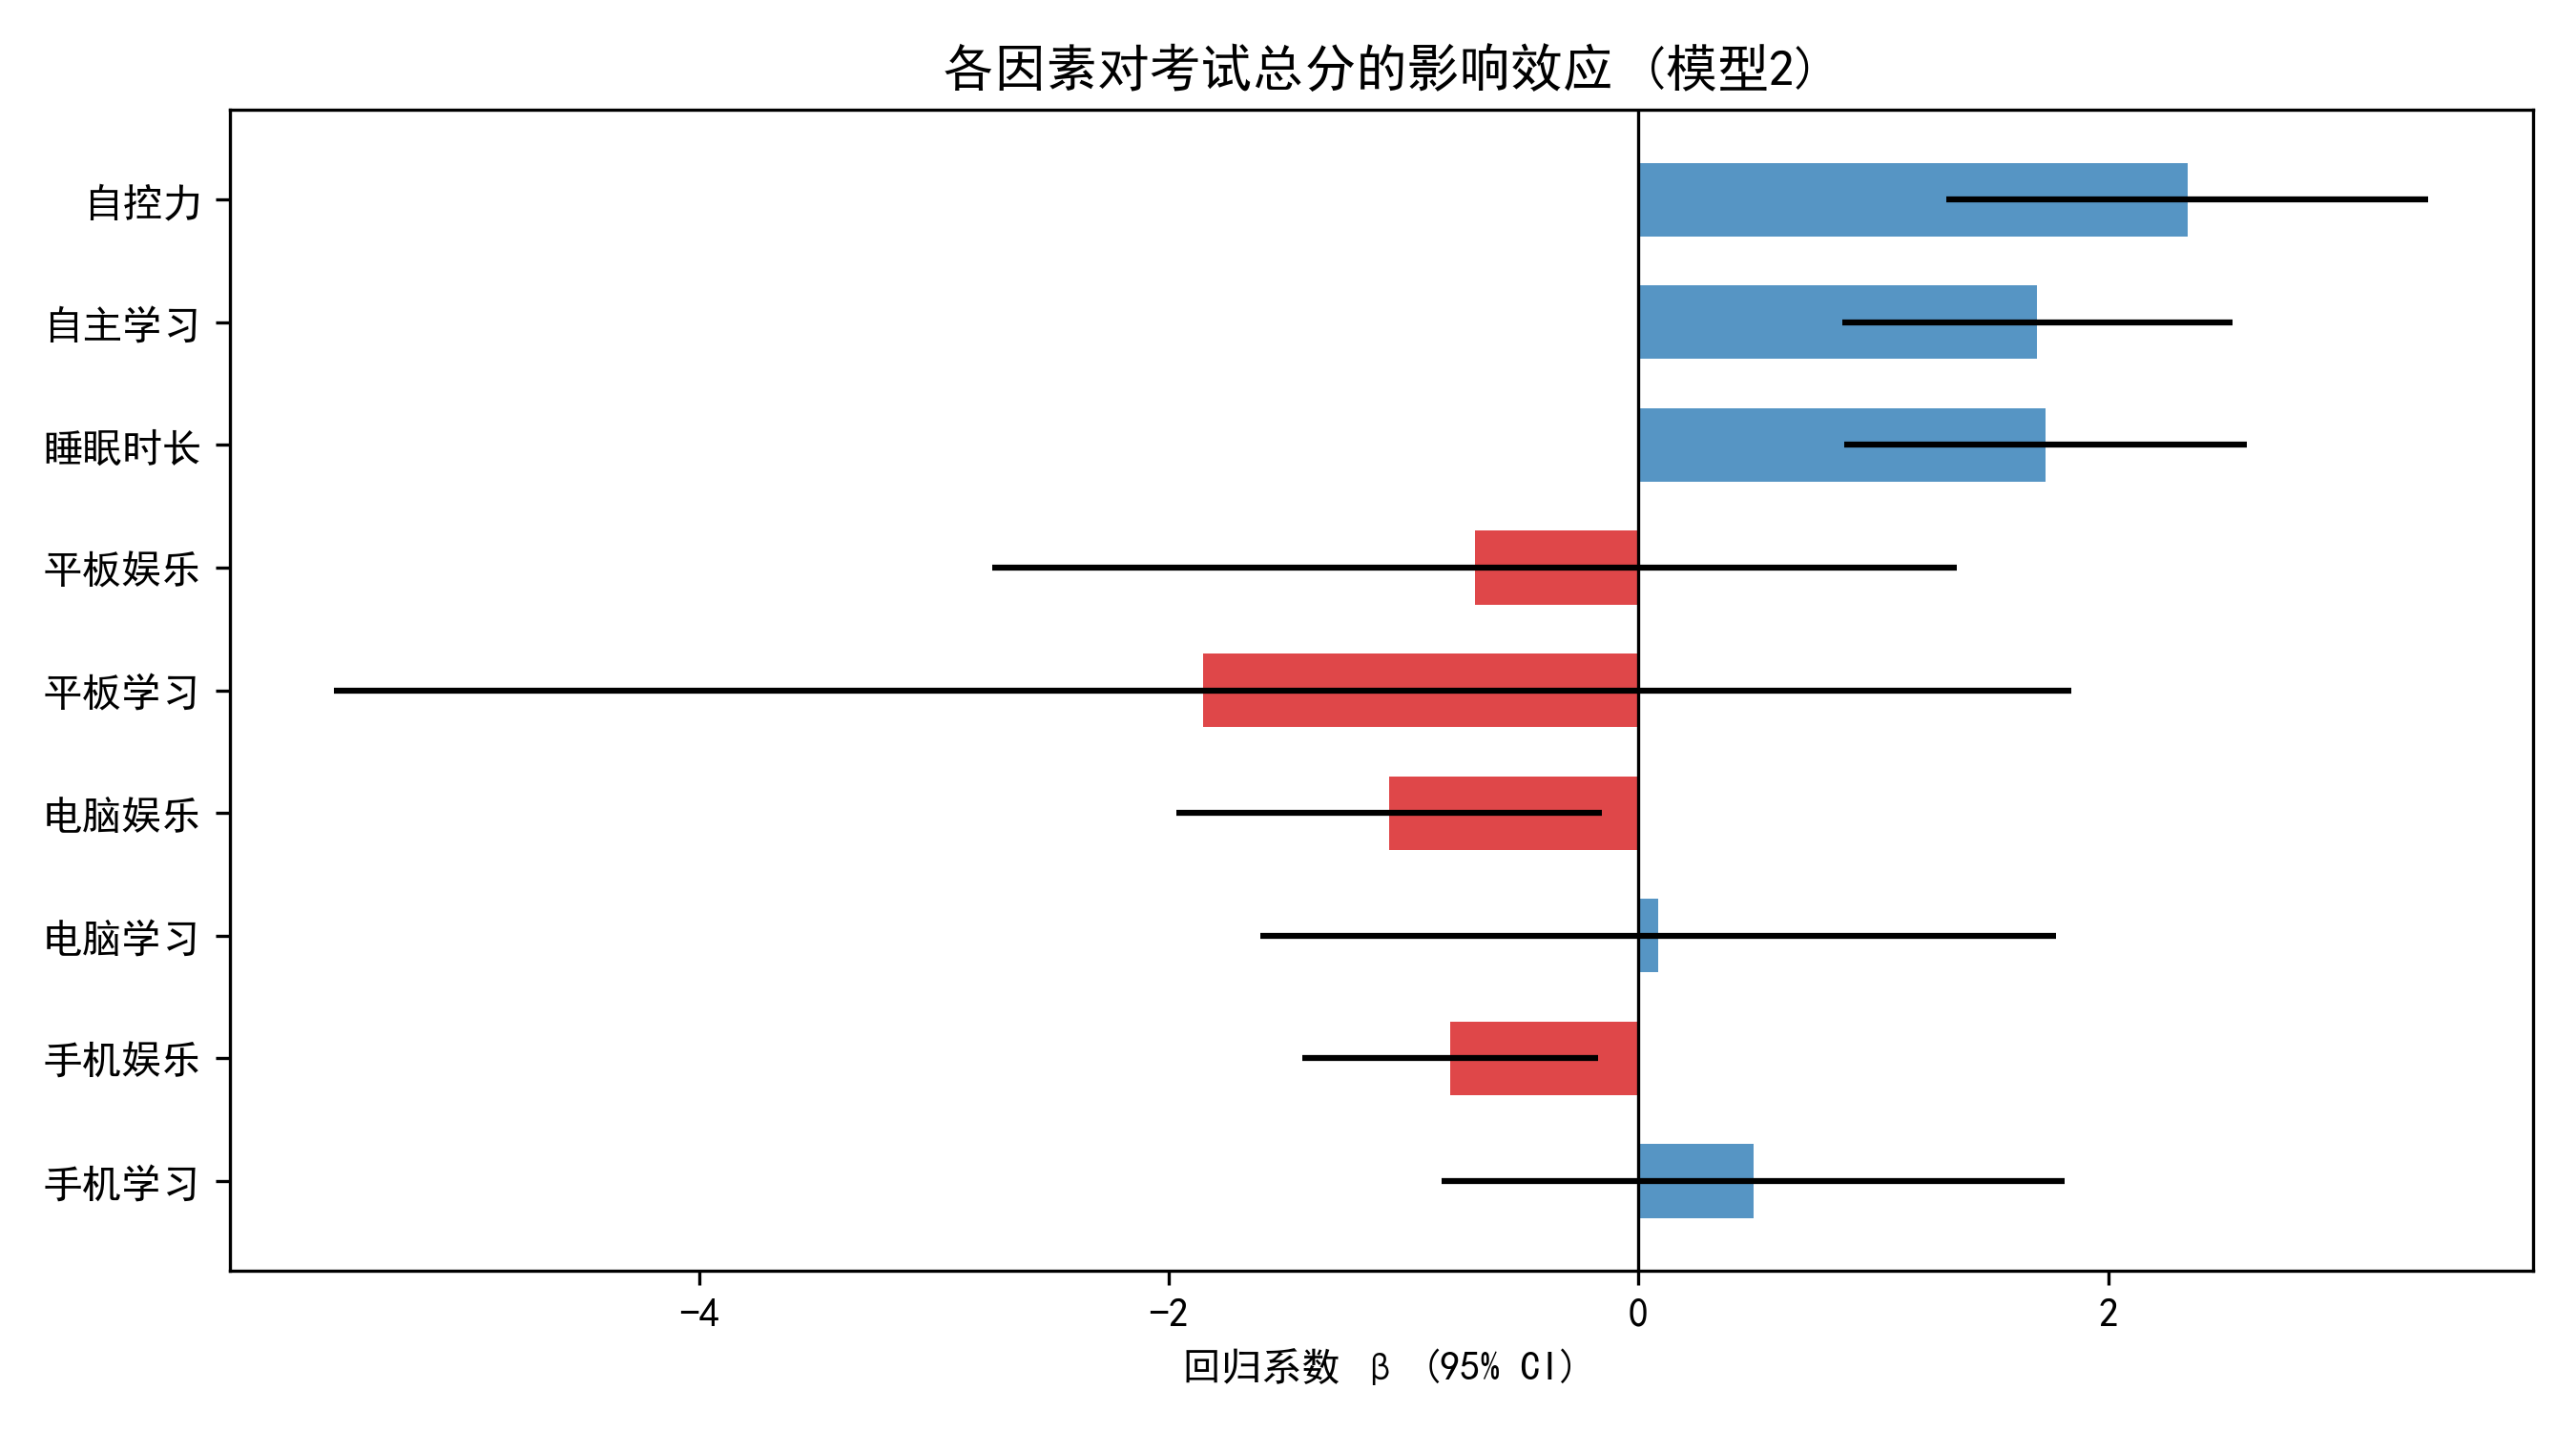
\includegraphics[width=0.95\textwidth]{fig_coefficient_forest.png}
\caption{各因素对考试总分的影响效应（模型2，95\% CI）}
\label{fig:forest}
\end{figure}

\subsection{Q5：结论与建议}

\subsubsection{核心发现}

\begin{enumerate}[leftmargin=*]
    \item \textbf{娱乐型电子设备使用对成绩存在显著但温和的负面影响}：手机娱乐（$\beta=-0.80$/h, $p=0.013$）和电脑娱乐（$\beta=-1.06$/h, $p=0.022$）均显著负向预测成绩，但效应量处于中等水平（Cohen's $f^2=0.23$）。控制学习习惯后该效应不降反升——说明即使在同样努力的学生中，娱乐使用更多的仍表现更差。
    \item \textbf{学习行为习惯比设备使用更重要}：仅设备使用变量几乎无法预测成绩（$R^2=3.3\%$），加入睡眠、自学和自控力后解释力提升5倍至19\%。在所有预测因子中，自控力的标准化效应最强（$\beta^*=+0.270$），其次为自主学习（$+0.238$）和睡眠（$+0.234$），最后才是娱乐使用（约$-0.14$）。
    \item \textbf{学习为目的的设备使用无显著效果}：用手机/电脑/平板学习的时长与成绩均无显著相关。这可能是因为（a）学习使用的测量受社会期望偏差影响；（b）"学习使用"的时间中混杂了娱乐切换；（c）有效学习更多取决于质量而非工具。
    \item \textbf{不应"一刀切"禁止电子设备}：鉴于设备使用的独立解释力仅3.3\%，简单禁止电子设备不太可能显著改善学业表现。更有效的方法是培养学生的睡眠习惯、自主学习能力和自控力。
\end{enumerate}

\subsubsection{分层建议}

\textbf{对学生}：（1）将每日手机娱乐时间控制在3小时以内——虽然效应量不大，但长期累积效应可观；（2）优先保障7.5小时以上的睡眠和2小时以上的自主学习——这两项的获益远大于减少娱乐使用；（3）警惕"用手机学习"的自我欺骗——本研究发现学习使用与成绩无显著关联。

\textbf{对家长}：（1）关注孩子的睡眠时间和自主学习习惯，这比管控设备使用更有效；（2）培养自控力（帮助制定计划、设置目标、逐步放权）是最具长期价值的干预；（3）管控设备使用时，重点限制娱乐使用（尤其是手机和电脑游戏），而非一概禁止所有电子设备。

\textbf{对学校}：（1）加强睡眠健康教育——睡眠时长在本研究中是第二强的正向预测因子；（2）开设时间管理和自控力训练课程；（3）避免"全校禁止带手机"的简单化政策——数据表明，问题的核心不是"有没有手机"，而是"怎么用"。

% ====== 6. 模型验证 ======
\section{模型验证与敏感性分析}

\subsection{Spearman秩相关稳健性检验}

由于设备使用变量偏态分布，以Spearman秩相关作为敏感性分析。Spearman $\rho$与Pearson $r$的方向和显著性完全一致，核心结论不变：

\begin{table}[H]
\centering
\caption{Pearson vs Spearman 稳健性对比}
\begin{tabular}{lrr}
\toprule
变量 & Pearson $r$ & Spearman $\rho$ \\
\midrule
手机-娱乐使用 & $-0.137^{*}$ & $-0.135^{*}$ \\
睡眠时长 & $+0.212^{***}$ & $+0.228^{***}$ \\
自主学习 & $+0.205^{**}$ & $+0.236^{***}$ \\
自控力 & $+0.193^{**}$ & $+0.204^{**}$ \\
\bottomrule
\end{tabular}
\end{table}

\subsection{模型增量解释力分析}

模型1到模型2的$F$检验：$F(3,240) = 15.52$, $p<0.001$，证实学习行为习惯变量的加入显著提升了模型解释力。$\Delta R^2=+0.157$表明成绩变异中的15.7\%由学习行为习惯独特解释，而设备使用仅能解释3.3\%。

% ====== 7. 模型评价 ======
\section{模型的评价与推广}

\subsection{优点与创新}

\begin{enumerate}[leftmargin=*]
    \item \textbf{完整的调查-分析链路}：从问卷设计、样本量计算到统计分析，完整展示了一项实证研究的全部环节
    \item \textbf{$3\times2$设备-目的矩阵}：精细化区分设备类型和使用目的，避免了将所有"屏幕时间"混为一谈的常见简化
    \item \textbf{偏相关揭示净效应}：通过偏相关分析区分了设备使用的独立效应与学习行为习惯的混淆效应
    \item \textbf{嵌套模型量化增量解释力}：通过模型1→模型2的$\Delta R^2$分析，量化了"设备使用vs学习习惯"的相对重要性——这一分析本身就构成了对"电子设备焦虑"的实证回应
    \item \textbf{方法有据、完全可复现}：正态性检验指导方法选择、多重诊断保证统计推断有效性、固定种子和开源代码确保可复现
\end{enumerate}

\subsection{局限与改进}

\begin{enumerate}[leftmargin=*]
    \item \textbf{模拟数据}：数据为基于合理假设的模拟生成，非真实调查数据，结论的效应量大小依赖生成模型中的参数设定。若实施真实调查，效应量可能与当前结果有所不同。但本研究展示的分析方法流程完全适用于真实数据。
    \item \textbf{横截面设计}：无法区分"设备使用→成绩"和"成绩→设备使用"（反向因果：成绩差→更多逃避→更多娱乐使用）。需要面板数据或工具变量法进行因果推断。
    \item \textbf{自我报告偏差}：设备使用时長的自我报告存在社会期望偏差和回忆偏差。未来可结合App使用记录等客观测量。
    \item \textbf{遗漏变量}：模型解释力仅为19\%，大量成绩变异未被解释（认知能力、教学质量、同伴效应等）。
\end{enumerate}

\subsection{推广方向}
若获取真实面板数据，可以：（1）使用固定效应模型控制个体异质性；（2）检验"最佳使用量"倒U型假说；（3）中介分析探究设备使用→睡眠/注意力→成绩的因果路径。

% ====== 参考文献 ======
\begin{thebibliography}{12}

\bibitem{cnnic2024}
中国互联网络信息中心(CNNIC).
\newblock \textit{2024年全国未成年人互联网使用情况研究报告}.
\newblock 北京: CNNIC, 2024.

\bibitem{oecd2022}
OECD.
\newblock \textit{PISA 2022 Results: Students' ICT Familiarity and Digital Learning}.
\newblock OECD Publishing, 2023.

\bibitem{cohen1988}
J. Cohen.
\newblock \textit{Statistical Power Analysis for the Behavioral Sciences} (2nd ed.).
\newblock Lawrence Erlbaum, 1988.

\bibitem{twenge2018}
J.~M.~Twenge, G.~N.~Martin, and W.~K.~Campbell.
\newblock Decreases in psychological well-being among American adolescents after 2012 and links to screen time.
\newblock \textit{Emotion}, 18(6):765--780, 2018.

\bibitem{odgers2020}
C.~L.~Odgers and M.~R.~Jensen.
\newblock Adolescent mental health in the digital age: Facts, fears, and future directions.
\newblock \textit{J. Child Psychology and Psychiatry}, 61(3):336--348, 2020.

\bibitem{przybylski2019}
A.~K.~Przybylski and N.~Weinstein.
\newblock Digital Screen Time Limits and Young Children's Psychological Well-Being.
\newblock \textit{Child Development}, 90(1):e56--e65, 2019.

\bibitem{harrell2015}
F.~E.~Harrell Jr.
\newblock \textit{Regression Modeling Strategies} (2nd ed.).
\newblock Springer, 2015.

\bibitem{pedhazur1997}
E.~J.~Pedhazur.
\newblock \textit{Multiple Regression in Behavioral Research} (3rd ed.).
\newblock Harcourt Brace, 1997.

\end{thebibliography}

% ====== 附录 ======
\newpage
\appendix
\section{核心代码（analyze.py 节选）}
\begin{lstlisting}[language=Python]
# 模型2: 设备使用 + 学习行为习惯
import statsmodels.api as sm
X = sm.add_constant(df[device_vars + control_vars])
model = sm.OLS(df['考试总分'], X).fit()
print(model.summary())

# 标准化系数（比较相对重要性）
X_std = (X - X.mean()) / X.std()
y_std = (y - y.mean()) / y.std()
beta_std = sm.OLS(y_std, sm.add_constant(X_std)).fit().params

# 偏相关分析
for var in device_vars:
    X_ctrl = sm.add_constant(df[['睡眠时长_小时','自主学习时长_小时','自控力_1到5']])
    resid_var = sm.OLS(df[var], X_ctrl).fit().resid
    resid_score = sm.OLS(df['考试总分'], X_ctrl).fit().resid
    r_partial, p_partial = pearsonr(resid_var, resid_score)
\end{lstlisting}

\section{代码文件清单}
\begin{itemize}
    \item \texttt{generate\_data.py} — 基于问卷框架生成模拟调查数据（SEED=42）
    \item \texttt{analyze.py} — 描述统计 + 相关性分析 + 回归建模 + 可视化
\end{itemize}
所有代码使用Python 3.x，依赖numpy, pandas, scipy, statsmodels, matplotlib, seaborn。

\textbf{⚠ 数据声明}：本研究中\texttt{survey\_data.csv}为模拟生成数据。若使用真实调查数据，只需替换该文件，本文所有分析代码无需修改即可复用。

\end{document}
